\documentclass[conference]{IEEEtran}
\IEEEoverridecommandlockouts

\usepackage{amsmath,amssymb,amsfonts}
\usepackage{algorithmic}
\usepackage{graphicx}
\usepackage{textcomp}
\usepackage{xcolor}

\usepackage[english]{babel}
\usepackage{csquotes}
\usepackage[
    backend=biber, 
    natbib=true,
    style=numeric,
    sorting=none,
]{biblatex}
\addbibresource{Bibliography.bib}


\ifCLASSOPTIONcompsoc                         \usepackage[caption=false,font=normalsize,labelfont=sf,textfont=sf]{subfig}
\else
\usepackage[caption=false,font=footnotesize]{subfig}
\fi


\def\BibTeX{{\rm B\kern-.05em{\sc i\kern-.025em b}\kern-.08em
    T\kern-.1667em\lower.7ex\hbox{E}\kern-.125em}}
    

\begin{document}

\title{
   Irrigation Control System Based On Fuzzy Logic
}

\author{
    \IEEEauthorblockN{  
    Ying Ying Lai
    }
    \IEEEauthorblockA{
        \textit{
            School of Information Technology
        }\\
        \textit{
            Monash University Malaysia
        }\\
        ylai0018@student.monash.edu
    }   
}
\maketitle



% #########################################
% ------------- INTRODUCTION -------------
% #########################################
\section{Introduction}
With the current technological advancements, Internet of Things (IoT) has been widely used in the field of machine learning and automation, especially when combined with Artificial Intelligence (AI) technologies. With the help of sensors, data collected can be sent to the server for statistical information and processing ~\cite{kokkonis_kontogiannis_tomtsis_2017}. One of the most popular application is smart irrigation systems, which play a huge role in tackling the global water crisis by reducing excess water use. It ensures optimal use of water, and at the same time increases production rate of crops. 

In this report, a fuzzy logic-based irrigation system is proposed to determine the length of time that the system must run to apply enough water to meet the plant watering requirement. The fuzzy control system has three input variables and one output variables. The input variables include soil moisture (\%), air humidity(\%) and temperature(ºC), meanwhile the output variables is the duration of valve opening (minutes). The advantage of using a fuzzy logic is its ability to handle uncertainty in lexical semantics. It works according to interval values, such as very long, long, medium, short and very short, as in human logic ~\cite{alpay_erdem_2018}.

\section{System Design}
The fuzzy logic irrigation control system consists of three state (input) variables and one control (output) variable. The unit, value range and linguistic variables of the inputs and outputs are shown in Table ~\ref{table:input_output}. The controller controls the amount of water to be watered by limiting the duration of the valve opening time. 

Firstly, a set of fuzzy rules will be determined. Then, the input will be made fuzzy using the input membership functions as shown in Table~\ref{table:moisture_mem}, Table~\ref{table:humidity_mem},Table~\ref{table:temperature_mem} and Table~\ref{table:duration_mem}. All five output membership functions are combined and finally a deffuzzified output distribution is obtained. An output value representing the duration of the valve opening time will be determined based on the input values.

 \begin{table}[!ht]
    \caption{State and Control Variables}
    \label{table:input_output}
    \centering
    \begin{tabular}{c c c c }
        \hline 
        \bfseries Type & \bfseries Variables & \bfseries Range & \bfseries Linguistic Variable  \\
        \hline  
          State & Soil Moisture & 0-100\% & L, M, H\\
           & Air Humidity & 0-100\% & L, M, H\\
           & Temperature & -10-50ºC & L, M, H\\
          \hline
          Control & Duration & 0-10min & VS, S, M, L, VL\\
    \hline
    \end{tabular}
\end{table}

\subsection{Membership Functions}
The membership functions for each state variable and control variable are provided in this section. The range are determined based on various studies on smart irrigation system ~\cite{kokkonis_kontogiannis_tomtsis_2017}~\cite{alpay_erdem_2018}~\cite{mohammed2021intelligent}~\cite{truneh2018fuzzy}.

 \begin{table}[!ht]
    \caption{Membership Functions of Soil Moisture}
    \label{table:moisture_mem}
    \centering
    \begin{tabular}{c c c}
        \hline 
        \bfseries Name of MF & \bfseries Membership Function & \bfseries MF Parameters\\
        \hline  
        Low (L) & Trapezoid-Shaped & [0, 0, 20, 40] \\
        Medium (M) & Triangle & [30, 50, 70]\\
        High (H) & Trapezoid-Shaped & [60, 80, 100, 100]\\
    \hline
    \end{tabular}
\end{table}

\begin{figure}[!ht]
    \centering
     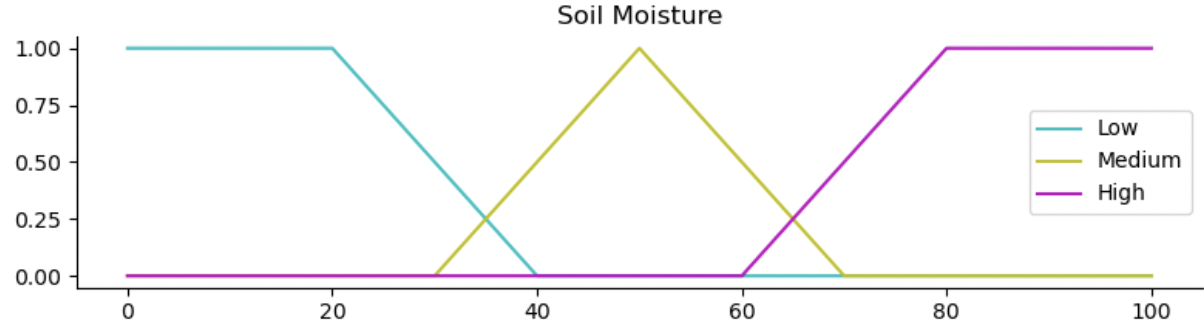
\includegraphics[width=3in]{graphs/moisture.png}
    \caption{Membership Functions For Soil Moisture} 
    \label{figure:moisture}
\end{figure}


 \begin{table}[!ht]
    \caption{Membership Functions of Air Humidity}
    \label{table:humidity_mem}
    \centering
    \begin{tabular}{c c c}
        \hline 
        \bfseries Name of MF & \bfseries Membership Function & \bfseries MF Parameters\\
        \hline  
        Low (L) & Trapezoid-Shaped & [0, 0, 15, 40] \\
        Medium (M) & Triangle & [25, 50, 75]\\
        High (H) & Trapezoid-Shaped & [60, 85, 100, 100]\\
    \hline
    \end{tabular}
\end{table}

\begin{figure}[!ht]
    \centering
     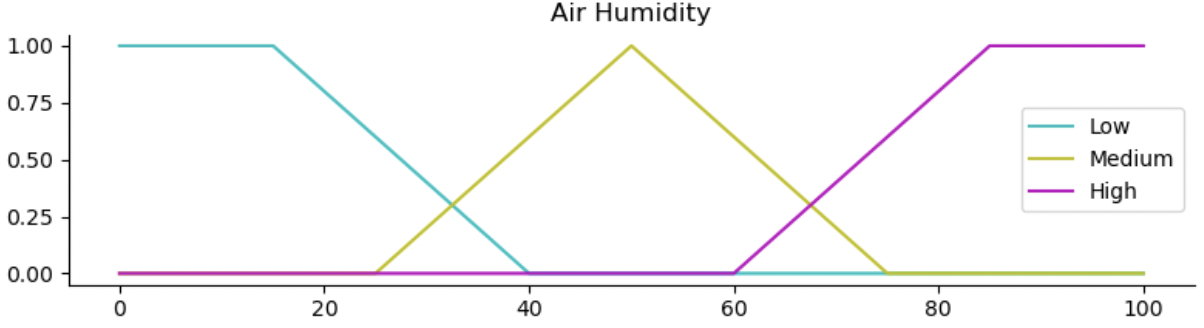
\includegraphics[width=3in]{graphs/humidity.png}
    \caption{Membership Functions For Air Humidity} 
    \label{figure:humidity}
\end{figure}



 \begin{table}[!ht]
    \caption{Membership Functions of Temperature}
    \label{table:temperature_mem}
    \centering
    \begin{tabular}{c c c}
        \hline 
        \bfseries Name of MF & \bfseries Membership Function & \bfseries MF Parameters\\
        \hline  
        Low (L)  & Trapezoid-Shaped & [-10, -10, 0, 15]\\
        Medium (M) & Triangle & [10, 20, 30]\\
        High (H) & Trapezoid-Shaped & [25, 40, 50, 50]\\
    \hline
    \end{tabular}
\end{table}

\begin{figure}[!ht]
    \centering
     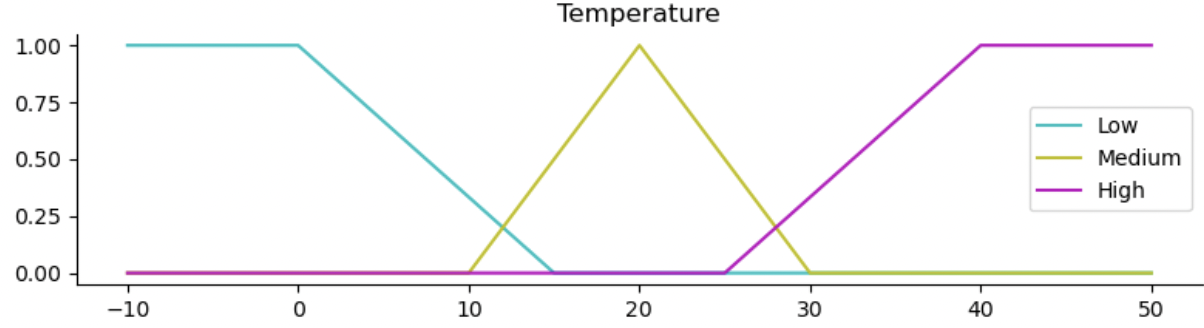
\includegraphics[width=3in]{graphs/temperature.png}
    \caption{Membership Functions For Temperature} 
    \label{figure:temperature}
\end{figure}

 \begin{table}[!ht]
    \caption{Membership Functions of Duration}
    \label{table:duration_mem}
    \centering
    \begin{tabular}{c c c}
        \hline 
        \bfseries Name of MF & \bfseries Membership Function & \bfseries MF Parameters\\
        \hline  
        Very Short (Vs) & Triangle & [0, 0, 2.5]\\
        Short (S) & Triangle & [0, 2.5, 5]\\
        Medium (M) & Triangle & [2.5, 5, 7.5]\\
        Long (L) & Triangle & [5, 7.5, 10]\\
        Very Long (VL) & Triangle & [7.5, 10, 10]\\
    \hline
    \end{tabular}
\end{table}

\begin{figure}[!ht]
    \centering
     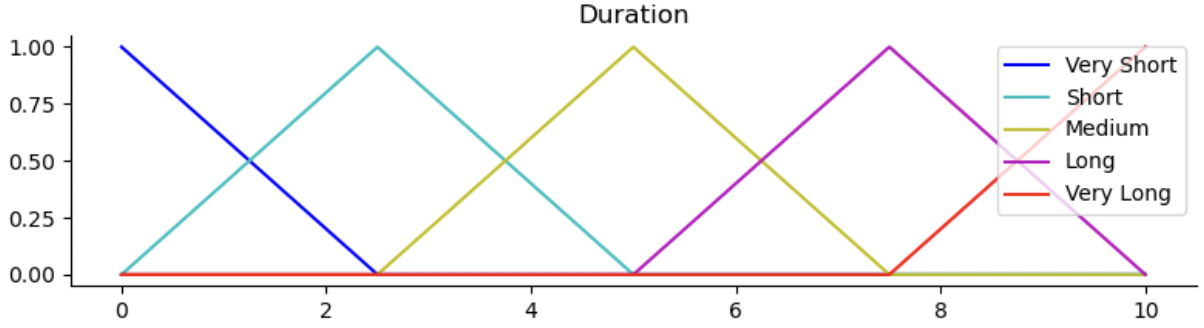
\includegraphics[width=3in]{graphs/duration.png}
    \caption{Membership Functions For Duration} 
    \label{figure:duration}
\end{figure}

\subsection{Fuzzy Rules}
Soil moisture, air humidity and temperature have three fuzzy variables each (Low (L), Medium (M) and High (H)), whereas the output variable, duration, has five fuzzy variables (very short (VS), short (S), medium (M), long (L), very long (VL)). 

\subsubsection{Rules of duration (in min) at low temperature}
 \begin{table}[!ht]
    \caption{Rules of duration (in min) at low temperature}
    \label{table:low_temp_rules}
    \centering
    \begin{tabular}{c  | c c c}
        \hline 
        \bfseries Soil Moisture & \bfseries & \bfseries  Air Humidity & \bfseries\\
                & Low   & Medium    & High\\
         \hline
        Low     & VL    & M         & S\\
        Medium  & M     & M         & S \\
        High    & S     & S         & VS\\
    \hline
    \end{tabular}
\end{table}

\subsubsection{Rules of duration (in min) at medium temperature}
 \begin{table}[!ht]
    \caption{Rules of duration (in min) at medium temperature}
    \label{table:medium_temp_rules}
    \centering
    \begin{tabular}{c  | c c c}
        \hline 
        \bfseries Soil Moisture & \bfseries & \bfseries  Air Humidity & \bfseries\\
                & Low   & Medium    & High\\
         \hline
        Low     & VL    & L         & M\\
        Medium  & L     & M         & S \\
        High    & M     & S         & VS\\
    \hline
    \end{tabular}
\end{table}

\subsubsection{Rules of duration (in min) at high temperature}
 \begin{table}[!ht]
    \caption{Rules of duration (in min) at high temperature}
    \label{table:high_temp_rules}
    \centering
    \begin{tabular}{c  | c c c}
        \hline 
        \bfseries Soil Moisture & \bfseries & \bfseries  Air Humidity & \bfseries\\
                & Low   & Medium    & High\\
         \hline
        Low     & VL    & L         & L\\
        Medium  & L     & M         & M \\
        High    & L     & M         & VS\\
    \hline
    \end{tabular}
\end{table}

\subsection{Defuzzification}
Defuzzification is achieved by applying the center of gravity method(centroid) from the fuzzification results to obtain the center of area under the curve. This method is widely used for fuzzification as it facilitates smooth transition of defuzzied values around output fuzzy region ~\cite{JAISWAL2020105537}.

\section{Example Output}
\subsection{Output 1}
Values for input and output variables: \\
Soil moisture: 20\% \\
Air Humidity: 15\% \\
Temperature: -5ºC \\
Duration: 9.17 minutes 
\begin{figure}[!ht]
    \centering
     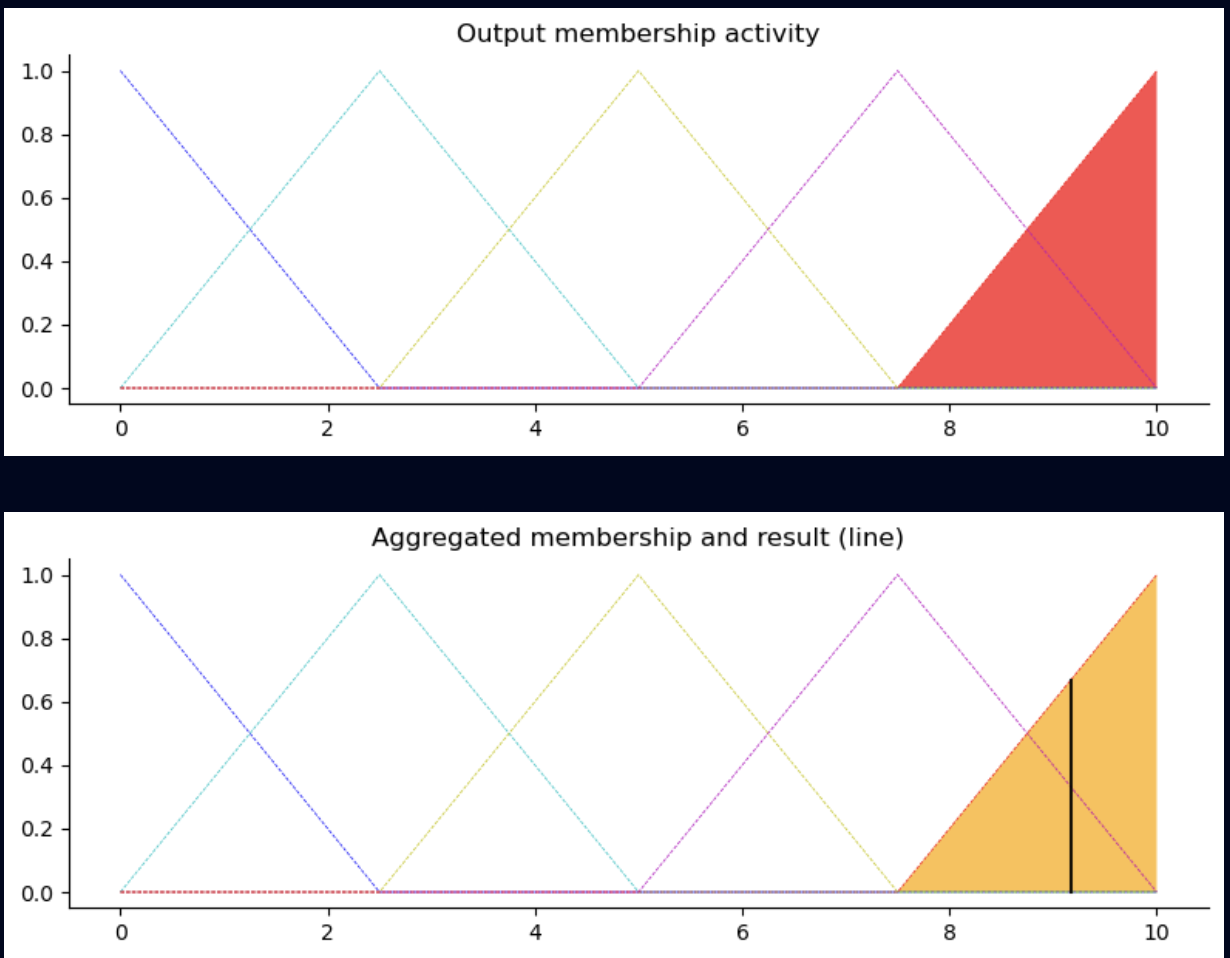
\includegraphics[width=3in]{graphs/20_15_-5.png}
    \caption{Output 1} 
\end{figure}

\subsection{Output 2}
Values for input and output variables: \\
Soil moisture: 40\% \\
Air Humidity: 3\% \\
Temperature: 5ºC \\
Duration: 5 minutes 
\begin{figure}[!ht]
    \centering
     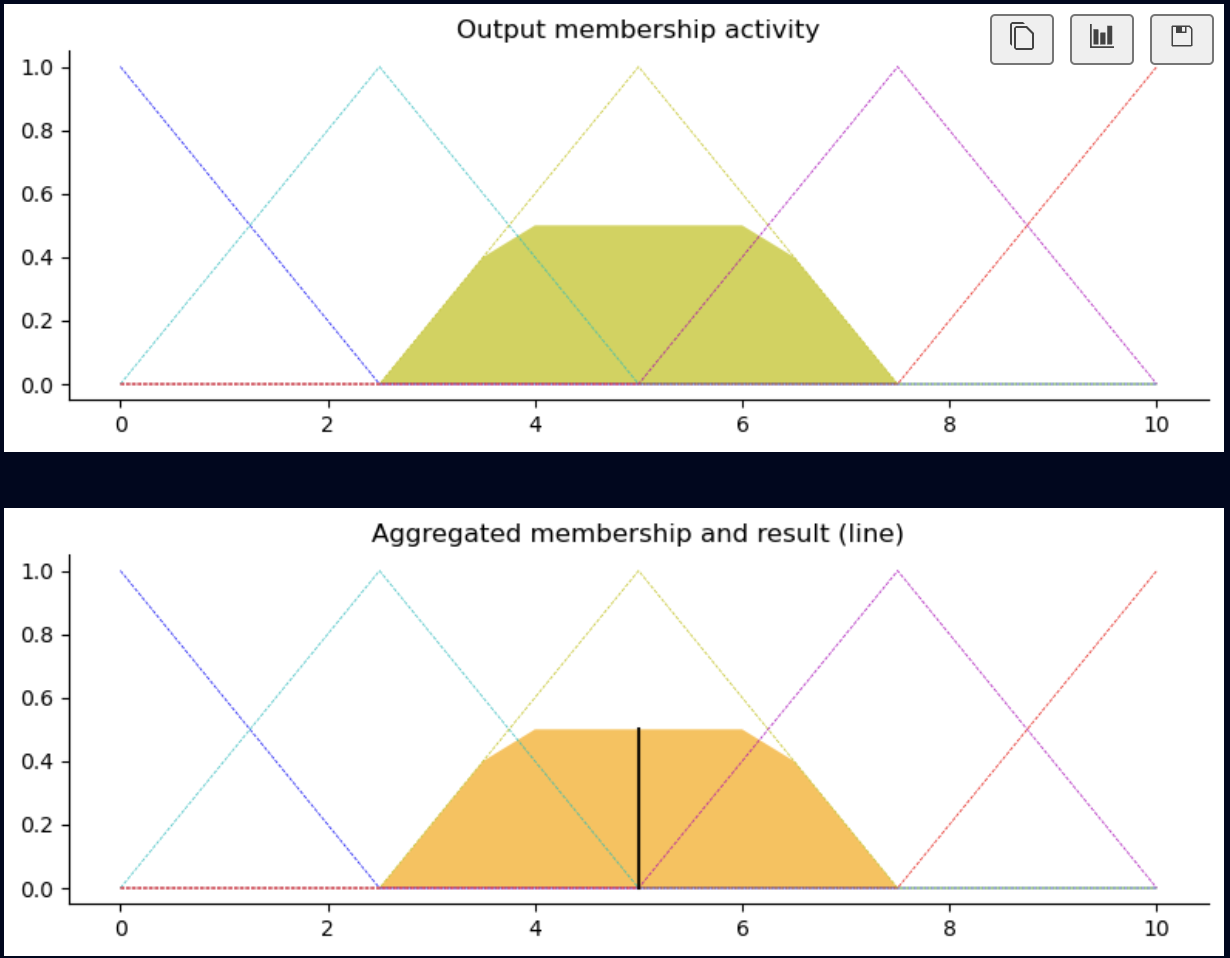
\includegraphics[width=3in]{graphs/40_3_5.png}
    \caption{Output 2} 
\end{figure}


\subsection{Output 3}
Values for input and output variables: \\
Soil moisture: 40\% \\
Air Humidity: 3\% \\
Temperature: 40ºC \\
Duration: 7.5 minutes 
\begin{figure}[!ht]
    \centering
     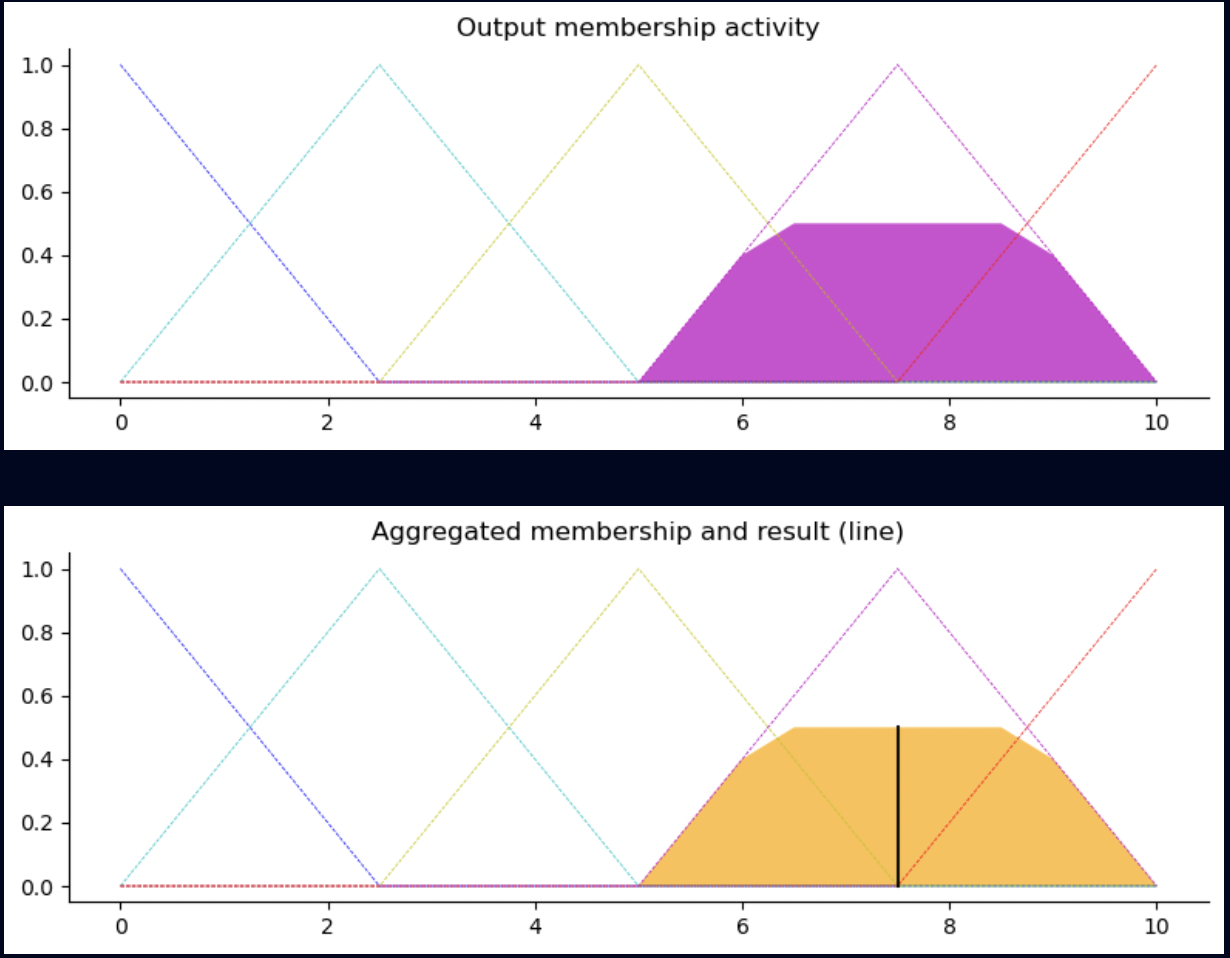
\includegraphics[width=3in]{graphs/40_3_40.png}
    \caption{Output 3} 
\end{figure}

\subsection{Output 4}
Values for input and output variables: \\
Soil moisture: 80\% \\
Air Humidity: 66\% \\
Temperature: 40ºC \\
Duration: 3.97  minutes 
\begin{figure}[!ht]
    \centering
     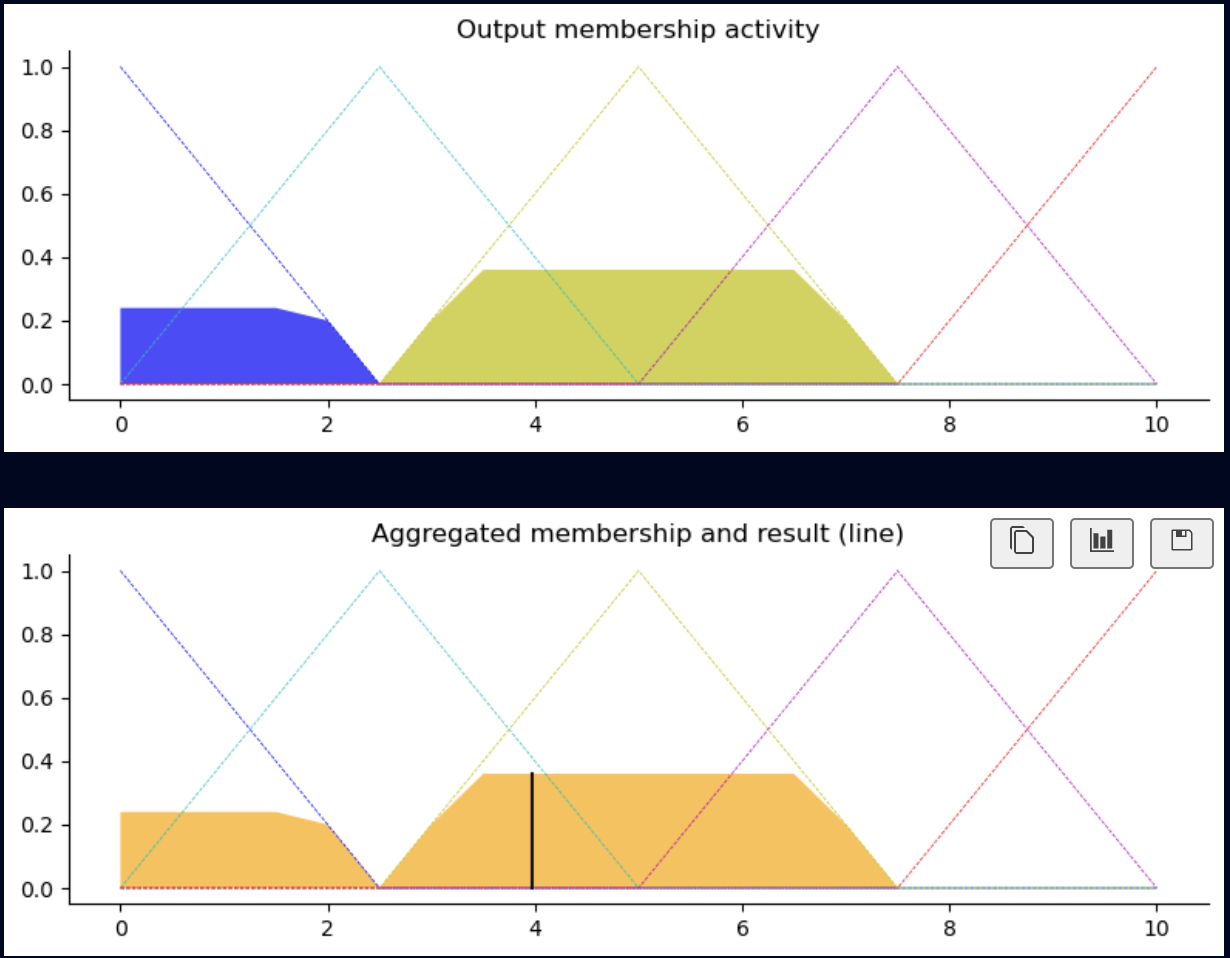
\includegraphics[width=3in]{graphs/80_66_40.png}
     \caption{Output 4} 
\end{figure}

\subsection{Output 5}
Values for input and output variables: \\
Soil moisture: 50\% \\
Air Humidity: 24\% \\
Temperature: 23ºC \\
Duration: 7.5  minutes 
\begin{figure}[!ht]
    \centering
     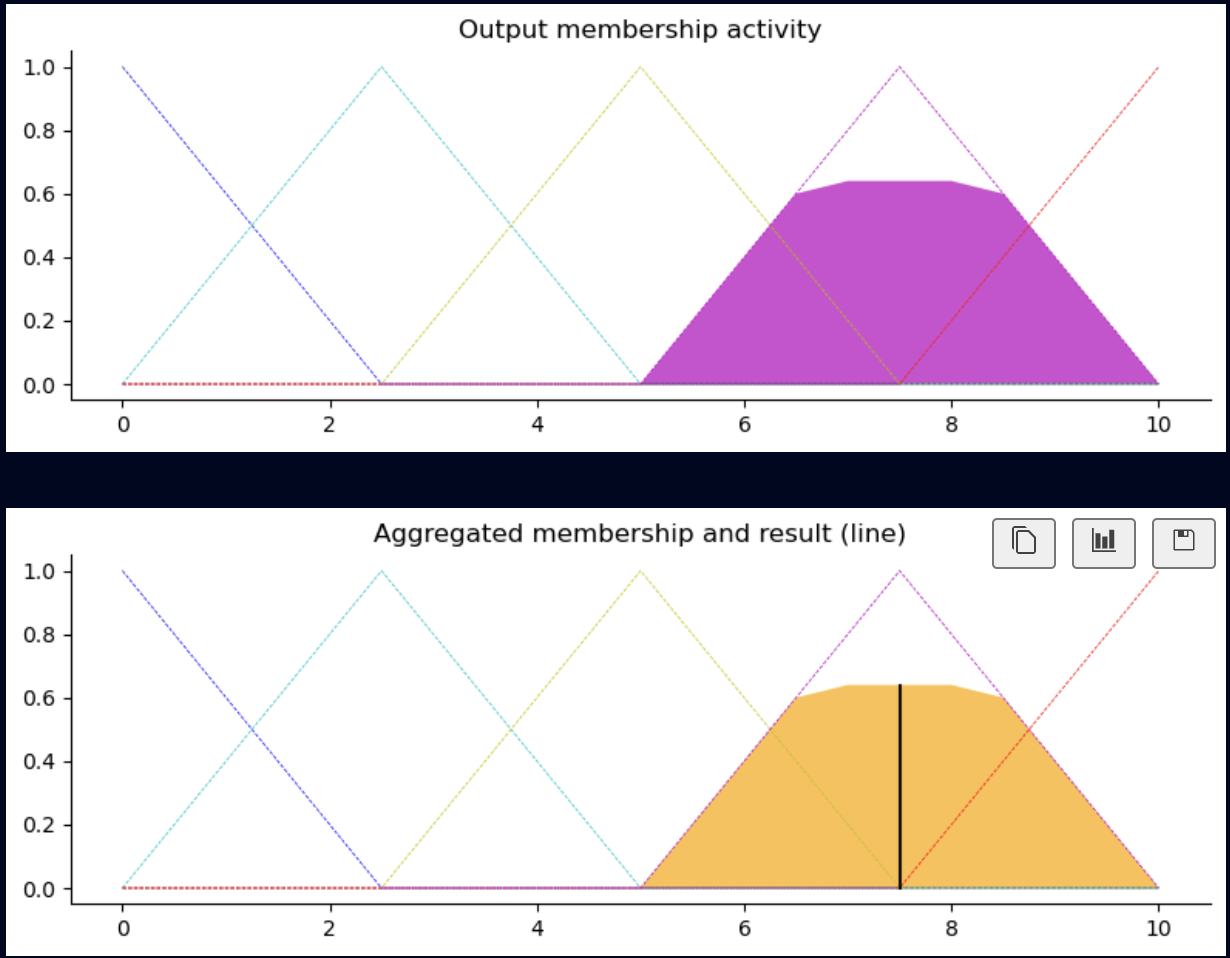
\includegraphics[width=3in]{graphs/50_24_23.png}
     \caption{Output 4} 
\end{figure}



\section{Discussions}
The advantages of applying Fuzzy inferences system in irrigation is the control system ensure optimal water usage by monitoring the soil moisture level, air humidity and temperature. No mathematical model is able to include all input parameters, hence, fuzzy logic technique is used since the membership functions are distributed based on the possible range of each state variable after fuzzification~\cite{truneh2018fuzzy}. By using fuzzy set theory, real life uncertainties can be handled effectively, which makes it an ideal choice for smart irrigation control system.

The limitation of this proposed model is that the fuzzy control system is only effective for a single type of crop. This is because the ideal range of the input variables is set according to the crop species.



\vspace{20pt}

\medskip

\printbibliography

\end{document}
